\documentclass[conference]{IEEEtran}
\IEEEoverridecommandlockouts

\usepackage{cite}
\usepackage{amsmath,amssymb,amsfonts,amsthm}
\usepackage{algorithm}
\usepackage{algorithmic}
\usepackage{graphicx}
\usepackage{textcomp}
\usepackage{xcolor}
\usepackage{colortbl}
\usepackage{booktabs}
\usepackage{multirow}
\usepackage{mathtools}
\usepackage{bm}
\usepackage{pifont}
\usepackage{url}
\usepackage{tikz}
\usetikzlibrary{positioning,arrows.meta,fit,calc}
\usepackage{pgfplots}
\pgfplotsset{compat=1.17}
\usepackage[hidelinks,breaklinks=true]{hyperref}

\definecolor{rowgray}{RGB}{245,245,245}
\definecolor{ourblue}{RGB}{31,94,163}
\definecolor{basegray}{RGB}{150,150,150}
\definecolor{posgreen}{RGB}{46,125,50}
\definecolor{negred}{RGB}{198,40,40}
\newcommand{\cmark}{\ding{51}}
\newtheorem{definition}{Definition}

\begin{document}

\title{Dual Spatial-Temporal Shapley Attribution for Explainable Anomaly Detection in Dynamic Social Graphs}

\author{\IEEEauthorblockN{Iyad Assaad Nekka\textsuperscript{1},
Hamida Seba\textsuperscript{2},
Khaled-Walid Hidouci\textsuperscript{1},
Karima Amrouche\textsuperscript{1}}
\IEEEauthorblockA{\textsuperscript{1}LCSI Laboratory, National Higher School of Computer Science (ESI), Algiers, Algeria\\
\{i\_nekka, w\_hidouci, k\_amrouche\}@esi.dz}
\IEEEauthorblockA{\textsuperscript{2}Universit\'e Claude Bernard Lyon 1, Lyon, France\\
hamida.lagraa@univ-lyon1.fr}}

\maketitle

\begin{abstract}
Transformer-based detectors such as TADDY find anomalous edges in dynamic social
graphs with high accuracy, but they give no reason for an alarm: the analyst gets
a score and nothing more. We present a post-hoc framework that wraps a trained,
frozen TADDY model and returns two attribution vectors for each flagged edge: a
\emph{spatial} vector that says which neighbour roles drove the score, and a
\emph{temporal} vector that says which snapshot carried the signal. The framework
adapts the GraphSVX Shapley surrogate to TADDY's windowed tokens through an
embedding-space perturbation that replaces masked tokens with the mean of the
active ones, instead of the misleading index-space masking. On three dynamic
social graph benchmarks, detection is unchanged ($\Delta$AUC $=0$). In a
controlled comparison on the same trained model, the framework gives the highest
Comprehensiveness of all baselines on every dataset (Random, Attention, Gradient,
Gradient$\times$Input; paired Wilcoxon $p<10^{-10}$) and the highest Fidelity on
UCI-Message, the dataset where Fidelity is not saturated. An ablation shows that
embedding-space masking is the component that matters: index-space masking cuts
Comprehensiveness by 41\%. An expanded evaluation over $2{,}621$ edges (true
positives, false positives and low-confidence detections) and a worked example
show how an analyst reads the two vectors. One explanation costs about 0.18\,s
on a CPU core.
\end{abstract}

\begin{IEEEkeywords}
Social network analysis, dynamic graphs, anomaly detection, explainability,
Shapley values, temporal attribution, graph transformers.
\end{IEEEkeywords}

% =============================================================================
\section{Introduction}
\label{sec:intro}
% =============================================================================

Social networks are never static. Messaging graphs, trust and rating
communities and platform interaction graphs change all the time as new edges
appear. Finding anomalous behaviour in these graphs (coordinated inauthentic
activity, abusive accounts, fraudulent ratings) is urgent in practice and hard
in theory \cite{akoglu2015graph}.

Deep detectors have raised accuracy a lot. NetWalk \cite{yu2018netwalk},
AddGraph \cite{zheng2019addgraph}, StrGNN \cite{cai2021strgnn} and TADDY
\cite{liu2021taddy} use graph neural networks and Transformers to capture
spatial and temporal patterns. TADDY stands out: it turns each candidate edge
into a short sequence of tokens (neighbour rank, hop distance and time step) and
feeds it to a BERT-style Transformer encoder. Benchmarks that re-run these
methods under one protocol place it among the strongest detectors
\cite{nekka2026survey}.

None of these detectors can explain itself. When edge $(u,v)$ is flagged at
snapshot $t$, TADDY returns a score. It does not say which of the surrounding
nodes looked suspicious, or whether the anomaly appeared now or was building
over earlier snapshots. Trust-and-safety teams cannot act on alerts they cannot
understand, and regulated settings require automated decisions to be justified.

For TADDY, explanation quality metrics are not low: they are
\emph{undefined}, because there is no attribution to evaluate. This paper fills
that gap. Our framework wraps a frozen TADDY model and, for each flagged edge,
answers two questions at once: \emph{was the alarm driven by a suspicious
counterparty, or by a suspicious moment in the interaction history?}

\noindent\textbf{Contributions.}
\begin{enumerate}
\item The first post-hoc explainability framework for TADDY-style detectors,
producing \textbf{dual spatial and temporal attribution vectors} for each
flagged edge, with zero change to detection.
\item A \textbf{graph-aware embedding-space perturbation} that replaces excluded
tokens with the mean embedding of the active coalition. An ablation shows it is
the essential component of the framework.
\item A \textbf{controlled comparison} against four baselines on the same
trained model, with bootstrap confidence intervals and paired Wilcoxon tests:
the framework has the highest Comprehensiveness on all three datasets.
\item An \textbf{expanded evaluation over $2{,}621$ edges} (all true positives,
false positives and low-confidence detections), a worked example, a top-$k$
sensitivity study and a cost analysis.
\end{enumerate}

% =============================================================================
\section{Related Work}
\label{sec:related}
% =============================================================================

\subsection{Anomaly Detection in Dynamic Graphs}
Early methods used hand-crafted signals. CM-Sketch \cite{ranshous2016scalable}
keeps approximate edge counts and flags outliers; SpotLight
\cite{eswaran2018spotlight} measures distances between graph sketches. Deep
methods followed: AddGraph \cite{zheng2019addgraph} combines a GCN with a GRU,
StrGNN \cite{cai2021strgnn} learns from enclosing subgraphs, and TADDY
\cite{liu2021taddy} puts spatial and temporal context into one Transformer.
GeneralDyG \cite{yang2025generaldyg} and GADY \cite{lou2023gady} push accuracy
further. A recent unified benchmark compares these families under one protocol
\cite{nekka2026survey}. None of these detectors explains its predictions.

\subsection{Explainability for Graph Neural Networks}
GNNExplainer \cite{ying2019gnnexplainer} learns a soft mask over edges and
features; PGExplainer \cite{luo2020pgexplainer} learns this mask with a shared
network. GraphSVX \cite{duval2021graphsvx} estimates Shapley values for GNNs
with a ``Smarter'' coalition sampler and a weighted least-squares surrogate, in
the spirit of KernelSHAP \cite{lundberg2017shap}. We extend GraphSVX to TADDY's
temporal tokens, which requires a new player definition, a new perturbation and
a dual aggregation.

\subsection{Explainability for Temporal and Dynamic GNNs}
T-GNNExplainer \cite{xia2023tgnnexplainer} searches for important past events
with Monte Carlo tree search, and TempME \cite{chen2023tempme} finds important
temporal motifs; both target continuous-time models. DyExplainer
\cite{wang2023dyexplainer} and TGIB \cite{seo2024tgib} build explanations into
training. Han \emph{et al.} \cite{han2026explainable} explain anomalies in
dynamic \emph{heterogeneous} graphs through relation evolution. None of these
applies to a frozen, discrete-snapshot token model such as TADDY.

% =============================================================================
\section{Preliminaries}
\label{sec:prelim}
% =============================================================================

\subsection{Dynamic Graphs and Anomaly Detection}

\begin{definition}[Dynamic Graph]
A dynamic graph is a sequence $\mathcal{G}=\{G_1,\ldots,G_T\}$ where each
$G_t=(V,E_t)$ shares the node set $V$ and has a time-varying edge set
$E_t\subseteq V\times V$.
\end{definition}

\begin{definition}[Edge-Level Anomaly Detection]
A scorer $f:(e,t)\mapsto[0,1]$ gives each edge $e=(u,v)\in E_t$ at snapshot
$t$ a score $s_{e,t}$. Edges above a threshold $\tau$ are flagged.
\end{definition}

\subsection{TADDY}
\label{subsec:taddy}
TADDY \cite{liu2021taddy} encodes each candidate edge $(u,v)$ as a sequence of
$D=(k+2)\times W$ tokens, where $k$ is the number of neighbours and $W$ the
lookback window. At each lookback step $l\in\{0,\ldots,W{-}1\}$ there are two
endpoint tokens ($u$, $v$) and the $k$ most important neighbours, ranked by
personalised PageRank. Each token sums three learned embeddings:
\begin{equation}
\mathbf{h}_{i,l}=\mathbf{E}_{\mathrm{pos}}[\mathrm{pos}_{i,l}]+
\mathbf{E}_{\mathrm{hop}}[\mathrm{hop}_{i,l}]+
\mathbf{E}_{\mathrm{time}}[\mathrm{time}_{i,l}].
\label{eq:embed}
\end{equation}
The token matrix $\mathbf{H}_e\in\mathbb{R}^{D\times d}$ goes through an
$L$-layer Transformer encoder, and the score is
\begin{equation}
s_{e,t}=\sigma\!\left(\mathbf{W}_c\cdot
\tfrac{1}{k+1}\textstyle\sum_{i=0}^{k}\mathbf{h}^{(L)}_i\right).
\label{eq:score}
\end{equation}

\subsection{Shapley Values}
For players $\mathcal{N}=\{1,\ldots,M\}$ and a value function
$v:2^{\mathcal{N}}\to\mathbb{R}$, the Shapley value of player $j$ is
\begin{equation}
\phi_j=\sum_{S\subseteq\mathcal{N}\setminus\{j\}}
\frac{|S|!\,(M{-}|S|{-}1)!}{M!}\bigl[v(S\cup\{j\})-v(S)\bigr].
\label{eq:shapley}
\end{equation}
Shapley values are the unique attribution that satisfies efficiency, symmetry,
linearity and the null-player axiom \cite{shapley1953value}. GraphSVX
\cite{duval2021graphsvx} approximates them with a surrogate weighted by the
Shapley kernel
$w(S)=\frac{M-1}{\binom{M}{|S|}\,|S|\,(M-|S|)}$ \cite{lundberg2017shap}.

% =============================================================================
\section{The Explainability Framework}
\label{sec:framework}
% =============================================================================

\subsection{Design Principles}
\noindent\textbf{Post-hoc, zero modification.} The framework wraps a trained,
frozen TADDY model. Weights, training and inference are untouched, so detection
is preserved exactly.

\noindent\textbf{Dual decomposition.} Attributions are aggregated along two
axes: \emph{spatial} (which token role: $u$, $v$, or the neighbour of PageRank
rank $r$) and \emph{temporal} (which lookback step).

\noindent\textbf{Graph-aware perturbation.} Masking happens in TADDY's dense
embedding space, not in its discrete index space
(Section~\ref{subsec:masking}). Fig.~\ref{fig:overview} shows the pipeline.

\begin{figure*}[!t]
\centering
\resizebox{\textwidth}{!}{%
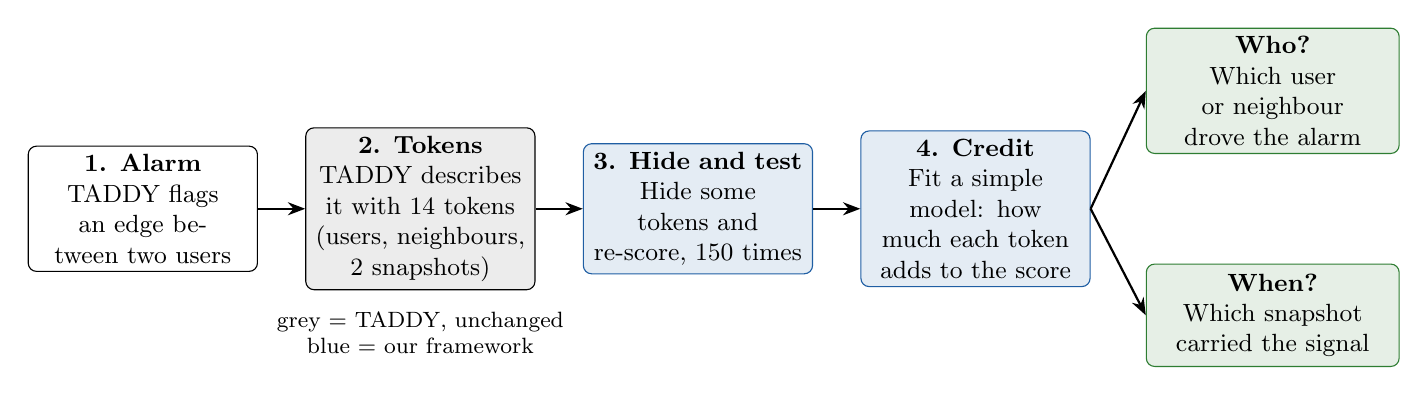
\begin{tikzpicture}[
  node distance=5mm and 6mm,
  stp/.style={draw, rounded corners=3pt, align=center, font=\small,
               minimum height=13mm, text width=27mm, inner sep=3pt, fill=white},
  frozen/.style={stp, fill=gray!15},
  ours/.style={stp, fill=ourblue!12, draw=ourblue},
  res/.style={stp, fill=posgreen!12, draw=posgreen, text width=30mm},
  arr/.style={-{Stealth[length=2.2mm]}, thick}]
\node[stp]   (a) {\textbf{1. Alarm}\\TADDY flags an edge between two users};
\node[frozen, right=of a] (b) {\textbf{2. Tokens}\\TADDY describes it with 14 tokens (users, neighbours, 2 snapshots)};
\node[ours,   right=of b] (c) {\textbf{3. Hide and test}\\Hide some tokens and re-score, 150 times};
\node[ours,   right=of c] (d) {\textbf{4. Credit}\\Fit a simple model: how much each token adds to the score};
\node[res, above right=-3mm and 7mm of d] (e) {\textbf{Who?}\\Which user or neighbour drove the alarm};
\node[res, below right=-3mm and 7mm of d] (f) {\textbf{When?}\\Which snapshot carried the signal};
\draw[arr] (a) -- (b); \draw[arr] (b) -- (c); \draw[arr] (c) -- (d);
\draw[arr] (d.east) -- (e.west); \draw[arr] (d.east) -- (f.west);
\node[font=\footnotesize, below=1.5mm of b, text width=58mm, align=center]
  {grey $=$ TADDY, unchanged \quad blue $=$ our framework};
\end{tikzpicture}}
\caption{How the framework works. TADDY stays unchanged. For each alarm, we hide
different groups of tokens, see how the score moves, and give each token its share
of the score. Adding up these shares by user role answers \emph{who}; adding them
up by snapshot answers \emph{when}.}
\label{fig:overview}
\end{figure*}

\subsection{Graph-Aware Coalition Masking}
\label{subsec:masking}
Index-space masking is misleading for TADDY: index $0$ in the intimacy-rank
table $\mathbf{E}_{\mathrm{pos}}$ is the \emph{highest-ranked} PageRank
neighbour, not a neutral token. Setting excluded indices to zero therefore
feeds the Transformer a strong neighbour signal for every excluded token and
biases the coalition scores.

We instead replace inactive tokens with the mean embedding of the active
coalition:
\begin{equation}
\tilde{\mathbf{h}}_j=\begin{cases}
\mathbf{h}_j & j\in S,\\
\bar{\mathbf{h}}_S=\frac{1}{|S|}\sum_{i\in S}\mathbf{h}_i & j\notin S.
\end{cases}
\label{eq:masking}
\end{equation}
The masked sequence skips EdgeEncoding and enters the Transformer directly. It
stays inside the convex hull of the active token embeddings, so the model sees
inputs close to its training distribution. This is the natural counterpart of
GraphSVX's neutral baseline for a token-based model, and the ablation in
Section~\ref{subsec:ablation} confirms that it matters.

\subsection{Algorithm}
Algorithm~\ref{alg:framework} gives the full procedure.

\begin{algorithm}[t]
\caption{Dual Spatial-Temporal Shapley Attribution}
\label{alg:framework}
\begin{algorithmic}[1]
\REQUIRE Trained TADDY (frozen); edge $e^*$; snapshot $t^*$; budget $N_s$
\ENSURE $\boldsymbol{\phi}_{\mathrm{spatial}}\in\mathbb{R}^{k+2}$,
        $\boldsymbol{\phi}_{\mathrm{temporal}}\in\mathbb{R}^{W}$
\STATE $s^*\leftarrow\sigma\bigl(\mathrm{TADDY\_logit}(e^*,t^*)\bigr)$
\STATE $\mathbf{H}\leftarrow\mathrm{EdgeEncoding}(e^*,t^*)\in\mathbb{R}^{D\times d}$
\STATE Sample $\mathbf{Z}\in\{0,1\}^{N_s\times D}$ (Smarter); kernel weights $\mathbf{w}$
\FOR{$i=1$ \TO $N_s$}
  \STATE $\tilde{\mathbf{H}}^{(i)}\leftarrow$ Eq.~\eqref{eq:masking} on
         $\mathbf{H}$ with mask $\mathbf{Z}[i,\cdot]$
  \STATE $f_i\leftarrow\sigma\bigl(\mathrm{Transformer\_logit}(\tilde{\mathbf{H}}^{(i)})\bigr)$
\ENDFOR
\STATE Fit kernel-weighted Ridge on $(\mathbf{Z},\mathbf{f},\mathbf{w})$;
       get $\hat{\boldsymbol{\beta}}\in\mathbb{R}^{D}$
\STATE $\phi_{\mathrm{spatial}}[r]\leftarrow\sum_{j:\,\mathrm{role}(j)=r}\hat{\beta}_j$ for each role $r$
\STATE $\phi_{\mathrm{temporal}}[l]\leftarrow\sum_{j:\,\mathrm{step}(j)=l}\hat{\beta}_j$ for each step $l$
\RETURN $\boldsymbol{\phi}_{\mathrm{spatial}},\,\boldsymbol{\phi}_{\mathrm{temporal}}$
\end{algorithmic}
\end{algorithm}

\subsection{Surrogate Fitting and Dual Decomposition}
The Smarter sampler always includes the full coalition $\mathbf{1}$ and the
empty coalition $\mathbf{0}$ (kernel weight capped at $10^3$, which enforces
efficiency in practice), then all $2D$ singleton perturbations (one token off,
one token on), and fills the rest of the budget with random coalitions. The
surrogate minimises
\begin{equation}
\hat{g}=\arg\min_{g}\sum_{i=1}^{N_s}w_i\bigl(g(\mathbf{Z}_i)-f_i\bigr)^2
+\lambda\|\boldsymbol{\beta}\|^2,
\label{eq:wls}
\end{equation}
and its coefficients $\hat{\boldsymbol{\beta}}$ are the approximate Shapley
values. Summing them by role and by step gives
\begin{equation}
\phi_{\mathrm{spatial}}[r]=\!\!\sum_{j:\,\mathrm{role}(j)=r}\!\!\hat{\beta}_j,
\qquad
\phi_{\mathrm{temporal}}[l]=\!\!\sum_{j:\,\mathrm{step}(j)=l}\!\!\hat{\beta}_j,
\label{eq:decomp}
\end{equation}
where $\mathrm{role}(j)\in\{u,v,n_1,\ldots,n_k\}$ and $n_r$ is the neighbour of
PageRank rank $r$. Endpoint tokens usually receive larger values because TADDY
pools the first $k{+}1$ tokens in Eq.~\eqref{eq:score}. The neighbour values
measure what each counterparty adds beyond the edge itself, which is the signal
an analyst needs for triage.

\subsection{Explanation Quality Metrics}
\label{subsec:metrics}
All metrics need an attribution vector; for TADDY alone they are undefined.
Let $s_{\mathrm{top}_k}$ be the score with only the $k$ highest-$|\hat\beta|$
tokens active, and $s_{\overline{\mathrm{top}_k}}$ the score with all tokens
\emph{except} them, both computed with Eq.~\eqref{eq:masking}. Following the
rationale literature \cite{deyoung2020eraser}:
\textbf{Fidelity} $\mathrm{Fid}=1-|s^*-s_{\mathrm{top}_k}|$;
\textbf{Sufficiency} $\mathrm{Suff}=s_{\mathrm{top}_k}$ (are the top-$k$ tokens
enough to keep the alarm?);
\textbf{Comprehensiveness} $\mathrm{Comp}=s^*-s_{\overline{\mathrm{top}_k}}$
(how much the score falls when they are removed; positive means they are
necessary); \textbf{Sparsity} $1-k/D$. All metrics are in probability space.

% =============================================================================
\section{Experiments}
\label{sec:experiments}
% =============================================================================

\subsection{Datasets and Setup}
We use three dynamic social graph benchmarks from the TADDY paper
\cite{liu2021taddy} (Table~\ref{tab:datasets}). Digg ($30{,}360$ nodes) was
left out because the spectral clustering used for anomaly injection exceeded
our memory budget.

\begin{table}[!t]
\centering
\caption{Datasets. Anomalies are synthetic cross-community edges injected at
10\% following TADDY's protocol \cite{liu2021taddy}.}
\label{tab:datasets}
\footnotesize
\setlength{\tabcolsep}{5pt}
\begin{tabular}{lrrrr}
\toprule
\textbf{Dataset} & \textbf{Nodes} & \textbf{Edges} &
\textbf{Snapshots} & \textbf{Anom.\ rate} \\
\midrule
UCI-Message   & 1{,}899 & 59{,}835 & 15 & 10\% \\
Bitcoin-Alpha & 3{,}783 & 24{,}186 & 15 & 10\% \\
Bitcoin-OTC   & 5{,}881 & 35{,}592 & 11 & 10\% \\
\bottomrule
\end{tabular}
\end{table}

\noindent\textbf{TADDY.} $k{=}5$, $W{=}2$, $d{=}32$, $L{=}2$ layers, $2$
heads, learning rate $10^{-3}$, weight decay $5{\times}10^{-4}$, $100$ epochs,
Adam, $50/50$ train/test snapshot split, seed $1$, all as in
\cite{liu2021taddy}. No tuning was done for the explainability study. The
Transformer was re-implemented in pure PyTorch for Python~3.12, with the same
architecture and training.

\noindent\textbf{Framework.} $N_s{=}150$ coalitions, top-$k{=}5$, $D{=}14$,
Ridge $\lambda{=}0.01$; sparsity is fixed at $1-5/14=0.643$.

\noindent\textbf{Baselines.} \emph{Random} (Gaussian scores);
\emph{Attention}: last-layer attention received per token, averaged over heads
\cite{jain2019attention}; \emph{Gradient}: $L_2$ norm of the gradient of $s^*$
with respect to each token embedding \cite{simonyan2014saliency};
\emph{Gradient$\times$Input}: sum over dimensions of gradient times embedding
\cite{shrikumar2017deeplift}. All methods are scored with the same metrics and
the same masking (Section~\ref{subsec:metrics}).

\noindent\textbf{Statistics.} We report 95\% bootstrap confidence intervals
($2{,}000$ resamples) and paired two-sided Wilcoxon signed-rank tests
\cite{wilcoxon1945} between our method and each alternative, pooled over the
$150$ explained edges. Code is publicly available.\footnote{\url{https://github.com/Iyad-Assaad-Nekka/Explainable-Taddy}}

\begin{table*}[!t]
\centering
\caption{Controlled comparison: every method explains the same 50
highest-scored true positives per dataset on the same trained TADDY models
($k{=}5$, $D{=}14$). Mean over edges; ``Avg'' is the mean of the three datasets.
$^{\dagger}$: our method is better with $p<0.01$ (paired Wilcoxon, 150 edges);
n.s.: $p\ge0.05$. Because this is a separate training run of the same
configuration, absolute values differ slightly from Tables~\ref{tab:gap},
\ref{tab:expanded} and \ref{tab:sensitivity}; the comparison \emph{within} this
table is what matters.}
\label{tab:baselines}
\footnotesize
\setlength{\tabcolsep}{4.2pt}
\begin{tabular}{l cccc cccc cccc}
\toprule
& \multicolumn{4}{c}{\textbf{Fidelity} $\uparrow$}
& \multicolumn{4}{c}{\textbf{Sufficiency} $\uparrow$}
& \multicolumn{4}{c}{\textbf{Comprehensiveness} $\uparrow$} \\
\cmidrule(lr){2-5}\cmidrule(lr){6-9}\cmidrule(lr){10-13}
\textbf{Method} & UCI & BTC-$\alpha$ & OTC & Avg
& UCI & BTC-$\alpha$ & OTC & Avg
& UCI & BTC-$\alpha$ & OTC & Avg \\
\midrule
Random            & 0.8711 & \textbf{0.9973} & 0.9983 & 0.9555 (n.s.)
                  & 0.8348 & 0.9916 & 0.9946 & 0.9403
                  & 0.0447 & $-$0.0002 & 0.0002 & 0.0149$^{\dagger}$ \\
Attention \cite{jain2019attention}
                  & 0.9002 & 0.9959 & 0.9978 & 0.9647$^{\dagger}$
                  & 0.8459 & \textbf{0.9953} & 0.9968 & 0.9460
                  & 0.1542 & 0.0006 & 0.0005 & 0.0518$^{\dagger}$ \\
Gradient \cite{simonyan2014saliency}
                  & 0.9157 & 0.9968 & 0.9984 & 0.9703$^{\dagger}$
                  & \textbf{0.9709} & 0.9943 & 0.9968 & \textbf{0.9873}
                  & 0.1530 & $-$0.0010 & 0.0002 & 0.0507$^{\dagger}$ \\
Grad$\times$Input \cite{shrikumar2017deeplift}
                  & 0.8704 & 0.9969 & \textbf{0.9995} & 0.9556$^{\dagger}$
                  & 0.8219 & 0.9943 & 0.9949 & 0.9370
                  & 0.1122 & 0.0002 & 0.0018 & 0.0381$^{\dagger}$ \\
\rowcolor{ourblue!10}
\textbf{Ours}     & \textbf{0.9342} & 0.9967 & 0.9980 & \textbf{0.9763}
                  & 0.9624 & 0.9945 & \textbf{0.9971} & 0.9847
                  & \textbf{0.1624} & \textbf{0.0169} & \textbf{0.0085} & \textbf{0.0626} \\
\midrule
\multicolumn{13}{l}{\textit{Ablation of our method}} \\
Index-space masking & 0.9033 & 0.9968 & 0.9987 & 0.9663 (n.s.)
                  & 0.8448 & 0.9944 & 0.9941 & 0.9444
                  & 0.1053 & 0.0040 & 0.0016 & 0.0370$^{\dagger}$ \\
Random sampler    & 0.9253 & 0.9967 & 0.9984 & 0.9735 (n.s.)
                  & 0.9676 & 0.9944 & 0.9967 & 0.9862
                  & 0.1814 & $-$0.0009 & 0.0046 & 0.0617$^{\dagger}$ \\
OLS (no kernel weights) & 0.9285 & 0.9968 & 0.9979 & 0.9744 (n.s.)
                  & 0.9746 & 0.9944 & 0.9972 & 0.9887
                  & 0.1927 & 0.0006 & 0.0060 & 0.0665 (n.s.) \\
\bottomrule
\end{tabular}
\end{table*}

\subsection{Detection Performance}

\begin{table}[!t]
\centering
\caption{AUC-ROC. The explainability layer leaves detection unchanged
($\Delta$AUC $=0$ by construction).}
\label{tab:auc}
\footnotesize
\setlength{\tabcolsep}{5pt}
\begin{tabular}{lccc}
\toprule
\textbf{Method} & \textbf{UCI} & \textbf{BTC-$\alpha$} & \textbf{BTC-OTC} \\
\midrule
TADDY \cite{liu2021taddy} (published) & 0.8370 & 0.9423 & 0.9425 \\
TADDY (our implementation)            & 0.8284 & 0.9554 & 0.9596 \\
\textbf{+ Explainability layer (ours)} & \textbf{0.8284} &
\textbf{0.9554} & \textbf{0.9596} \\
\bottomrule
\end{tabular}
\end{table}

Our re-implementation stays within $0.009$--$0.017$ AUC of the published
numbers (Table~\ref{tab:auc}). Table~\ref{tab:gap} is the starting point of
this work: before it, no explanation metric can be computed for TADDY.

\begin{table}[!t]
\centering
\caption{Explainability introduced. N/A $=$ undefined: TADDY produces no
attribution, so no metric can be computed. Mean over the top-50 true positives
of each dataset, averaged across the three datasets.}
\label{tab:gap}
\footnotesize
\setlength{\tabcolsep}{4pt}
\begin{tabular}{lccc}
\toprule
\textbf{Capability / Metric} & \textbf{TADDY} &
\textbf{+ Expl.\ (ours)} & \textbf{Status} \\
\midrule
\rowcolor{rowgray}
Fidelity             & N/A & \textbf{0.9562} & Introduced \\
Sufficiency          & N/A & \textbf{0.9658} & Introduced \\
\rowcolor{rowgray}
Comprehensiveness    & N/A & \textbf{0.0576} & Introduced \\
Spatial attribution  & N/A & \cmark          & Introduced \\
\rowcolor{rowgray}
Temporal attribution & N/A & \cmark          & Introduced \\
Coalitions evaluated per edge & 0 & 150      & --- \\
\bottomrule
\end{tabular}
\end{table}

\subsection{Comparison with Baselines}
\label{subsec:baselines}

Table~\ref{tab:baselines} compares all methods on the \emph{same} trained models
and the same top-50 true positives of each dataset. Fig.~\ref{fig:uci} shows
UCI-Message with confidence intervals.


\begin{figure}[!t]
\centering
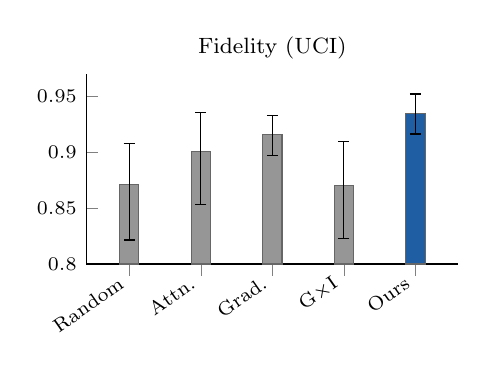
\begin{tikzpicture}
\begin{axis}[
  width=0.52\columnwidth, height=40mm,
  ybar, bar width=7pt, bar shift=0pt,
  symbolic x coords={Rnd,Att,Grad,GxI,Ours},
  xtick={Rnd,Att,Grad,GxI,Ours}, xticklabels={Random,Attn.,Grad.,G$\times$I,Ours}, xticklabel style={font=\scriptsize, rotate=35, anchor=east},
  ymin=0.80, ymax=0.97, ytick={0.80,0.85,0.90,0.95},
  yticklabel style={font=\scriptsize, /pgf/number format/fixed, /pgf/number format/precision=2},
  title={\footnotesize Fidelity (UCI)}, title style={yshift=-1.5mm},
  axis lines*=left, enlarge x limits=0.15]
\addplot[fill=basegray, draw=black!60,
  error bars/.cd, y dir=both, y explicit, error bar style={black}]
coordinates {
 (Rnd,0.8711) += (0,0.0368) -= (0,0.0496)
 (Att,0.9002) += (0,0.0349) -= (0,0.0470)
 (Grad,0.9157) += (0,0.0171) -= (0,0.0186)
 (GxI,0.8704) += (0,0.0388) -= (0,0.0480)};
\addplot[fill=ourblue, draw=black!60,
  error bars/.cd, y dir=both, y explicit, error bar style={black}]
coordinates {(Ours,0.9342) += (0,0.0176) -= (0,0.0181)};
\end{axis}
\end{tikzpicture}%
\hfill
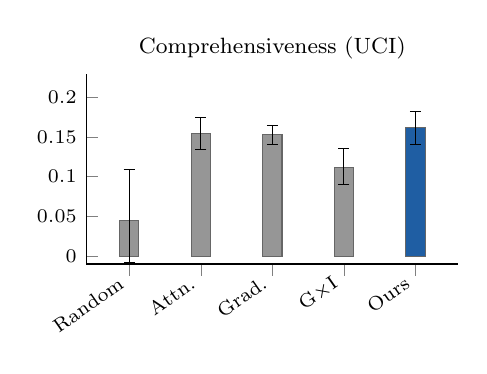
\begin{tikzpicture}
\begin{axis}[
  width=0.52\columnwidth, height=40mm,
  ybar, bar width=7pt, bar shift=0pt,
  symbolic x coords={Rnd,Att,Grad,GxI,Ours},
  xtick={Rnd,Att,Grad,GxI,Ours}, xticklabels={Random,Attn.,Grad.,G$\times$I,Ours}, xticklabel style={font=\scriptsize, rotate=35, anchor=east},
  ymin=-0.01, ymax=0.23, ytick={0,0.05,0.10,0.15,0.20},
  yticklabel style={font=\scriptsize, /pgf/number format/fixed, /pgf/number format/precision=2},
  title={\footnotesize Comprehensiveness (UCI)}, title style={yshift=-1.5mm},
  axis lines*=left, enlarge x limits=0.15]
\addplot[fill=basegray, draw=black!60,
  error bars/.cd, y dir=both, y explicit, error bar style={black}]
coordinates {
 (Rnd,0.0447) += (0,0.0649) -= (0,0.0532)
 (Att,0.1542) += (0,0.0204) -= (0,0.0193)
 (Grad,0.1530) += (0,0.0116) -= (0,0.0119)
 (GxI,0.1122) += (0,0.0230) -= (0,0.0219)};
\addplot[fill=ourblue, draw=black!60,
  error bars/.cd, y dir=both, y explicit, error bar style={black}]
coordinates {(Ours,0.1624) += (0,0.0193) -= (0,0.0213)};
\end{axis}
\end{tikzpicture}
\caption{UCI-Message, the dataset where the metrics are not saturated. Bars:
mean over the top-50 true positives; whiskers: 95\% bootstrap interval. Our method (blue) has the highest Fidelity
and Comprehensiveness.}
\label{fig:uci}
\end{figure}

Three results stand out.

\noindent\textbf{(i) Comprehensiveness.} Our method has the highest
Comprehensiveness on \emph{all three} datasets, and the gap is significant
against every baseline ($p\le2.3\times10^{-11}$). Removing the tokens it selects
lowers the score more than removing the tokens chosen by attention or
gradients, so its top tokens are the most \emph{necessary} ones.

\noindent\textbf{(ii) Fidelity.} Our method has the best average Fidelity and is
significantly better than Attention ($p=3.7\times10^{-5}$), Gradient
($p=6.1\times10^{-3}$) and Gradient$\times$Input ($p=3.9\times10^{-3}$). The
difference with Random is not significant ($p=0.25$), and the reason is
informative: on both Bitcoin datasets \emph{every} method, including Random,
reaches Fidelity $\approx0.997$. There the top-alarm edges are scored near $1$
from almost any subset of tokens, so Fidelity cannot separate methods. On UCI,
where it can, our method leads ($0.934$ vs.\ $0.916$ for the best baseline).

\noindent\textbf{(iii) Sufficiency.} Gradient is slightly higher on average
($0.987$ vs.\ $0.985$), mostly on UCI. Sufficiency rewards tokens that
\emph{keep} the score high; Comprehensiveness rewards tokens whose removal
\emph{lowers} it. Our method gives the best balance of the two.

\subsection{Ablation}
\label{subsec:ablation}
The lower block of Table~\ref{tab:baselines} removes one component at a time.

\noindent\textbf{Embedding-space masking is essential.} With index-space masking
(excluded indices set to $0$), Comprehensiveness drops by 41\% ($0.063\to0.037$,
$p=8.8\times10^{-17}$), and Sufficiency on UCI drops from $0.962$ to $0.845$.
This confirms the analysis of Section~\ref{subsec:masking}: index $0$ is not
neutral.

\noindent\textbf{The sampler and the kernel weights matter much less.} A plain
random sampler gives similar Fidelity and slightly lower Comprehensiveness
($p=3.2\times10^{-3}$), mainly because it turns negative on Bitcoin-Alpha.
Dropping the kernel weights (OLS) gives statistically indistinguishable results
(Comprehensiveness $p=0.67$). These parts are therefore replaceable; we keep
them because they follow the standard Shapley estimator
\cite{lundberg2017shap,duval2021graphsvx} and preserve its efficiency anchor.

\subsection{Expanded Evaluation Across Edge Categories}

Table~\ref{tab:expanded} evaluates four edge categories. The groups overlap:
``Top-50 TP'' and ``Low-Conf TP'' are subsets of ``All TP'', so the evaluation
covers $2{,}471$ distinct true positives and $150$ false positives, i.e.
$2{,}621$ distinct edges.

\begin{table}[!t]
\centering
\caption{Fidelity across edge categories. FP $=$ false positives (highest-scored
normal edges); Low-Conf TP $=$ true anomalies with the lowest scores. Top-50 TP
and Low-Conf TP are subsets of All TP: $2{,}471$ distinct TP $+$ $150$ FP
$=2{,}621$ distinct edges.}
\label{tab:expanded}
\footnotesize
\setlength{\tabcolsep}{4pt}
\begin{tabular}{llrcc}
\toprule
\textbf{Dataset} & \textbf{Category} & \textbf{n} &
\textbf{Fidelity} & \textbf{$\pm$Std} \\
\midrule
\rowcolor{rowgray}
UCI   & Top-50 TP   &   50 & 0.8743 & 0.222 \\
UCI   & All TP      &  691 & 0.9023 & 0.159 \\
\rowcolor{rowgray}
UCI   & FP          &   50 & 0.8428 & 0.281 \\
UCI   & Low-Conf TP &   50 & 0.8101 & 0.352 \\
\midrule
\rowcolor{rowgray}
BTC-$\alpha$ & Top-50 TP   &   50 & 0.9957 & 0.001 \\
BTC-$\alpha$ & All TP      &  706 & 0.9598 & 0.114 \\
\rowcolor{rowgray}
BTC-$\alpha$ & FP          &   50 & 0.9957 & 0.001 \\
BTC-$\alpha$ & Low-Conf TP &   50 & 0.9893 & 0.031 \\
\midrule
\rowcolor{rowgray}
BTC-OTC & Top-50 TP   &   50 & 0.9982 & 0.001 \\
BTC-OTC & All TP      & 1074 & 0.9735 & 0.095 \\
\rowcolor{rowgray}
BTC-OTC & FP          &   50 & 0.9977 & 0.001 \\
BTC-OTC & Low-Conf TP &   50 & 0.8158 & 0.300 \\
\midrule
\multicolumn{2}{l}{\textbf{Distinct edges}} & \textbf{2{,}621} & & \\
\bottomrule
\end{tabular}
\end{table}

\noindent\textbf{(i) Beyond the top-50.} Fidelity on all true positives stays
high ($0.902$--$0.974$), so the results do not depend on picking the most
confident alarms.

\noindent\textbf{(ii) False positives.} Fidelity on false alarms is
$0.843$ on UCI and $\ge0.996$ on the Bitcoin datasets. The framework can
therefore explain \emph{why} TADDY flagged a normal edge, which is what an
analyst needs to clear a false alarm quickly.

\noindent\textbf{(iii) Borderline detections.} Fidelity on low-confidence true
positives is $0.810$--$0.989$, lower and more variable than on confident ones,
as expected near the decision boundary.

\noindent\textbf{(iv) Comprehensiveness by category.} The value $0.0576$ in
Table~\ref{tab:gap} is the mean over the top-50 true positives of the three
datasets. In the controlled run (Table~\ref{tab:baselines}) it is positive on
every dataset ($0.162$, $0.017$, $0.009$). The one negative value we observed is
for low-confidence true positives on Bitcoin-Alpha ($-0.3995$), discussed in
Section~\ref{subsec:borderline}.

\subsection{Sensitivity to the Top-$k$ Budget}

\begin{table}[!t]
\centering
\caption{Fidelity of our method for $k\in\{3,5,7,10\}$ (top-50 TP). It rises
with $k$ on UCI; it is near saturation on the Bitcoin datasets.}
\label{tab:sensitivity}
\footnotesize
\setlength{\tabcolsep}{6pt}
\begin{tabular}{lcccc}
\toprule
\textbf{Dataset} & $k{=}3$ & $k{=}5$ & $k{=}7$ & $k{=}10$ \\
\midrule
UCI-Message    & 0.8578 & 0.8720 & 0.8976 & 0.9454 \\
Bitcoin-Alpha  & 0.9951 & 0.9957 & 0.9961 & 0.9975 \\
Bitcoin-OTC    & 0.9994 & 0.9982 & 0.9981 & 0.9988 \\
\bottomrule
\end{tabular}
\end{table}

Table~\ref{tab:sensitivity} shows that Fidelity on UCI rises steadily with $k$,
which is what a correct token ranking should produce: adding the next-best
tokens brings the score closer to the full-context score.

\subsection{Worked Example}

Fig.~\ref{fig:example} shows the explanation of the highest-scored true anomaly
on UCI-Message ($s^*=0.9965$).

\begin{figure}[!t]
\centering
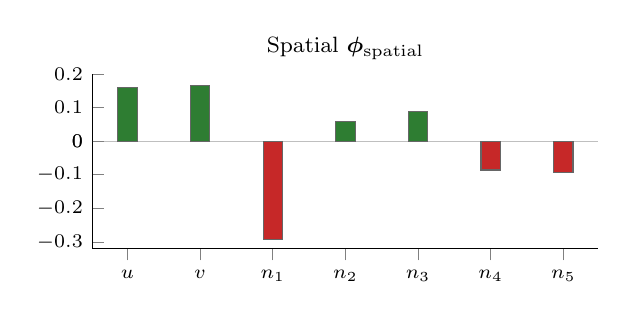
\begin{tikzpicture}
\begin{axis}[
  width=0.66\columnwidth, height=38mm,
  ybar, bar width=7pt, bar shift=0pt,
  symbolic x coords={u,v,n1,n2,n3,n4,n5},
  xtick={u,v,n1,n2,n3,n4,n5},
  xticklabels={$u$,$v$,$n_1$,$n_2$,$n_3$,$n_4$,$n_5$}, xticklabel style={font=\scriptsize},
  ymin=-0.32, ymax=0.20, ytick={-0.3,-0.2,-0.1,0,0.1,0.2},
  yticklabel style={font=\scriptsize, /pgf/number format/fixed, /pgf/number format/precision=1},
  title={\footnotesize Spatial $\boldsymbol\phi_{\mathrm{spatial}}$}, title style={yshift=-1.5mm},
  axis lines*=left, extra y ticks={0}, extra y tick style={grid=major},
  enlarge x limits=0.08]
\addplot[fill=posgreen, draw=black!60] coordinates {(u,0.1610) (v,0.1649) (n2,0.0575) (n3,0.0878)};
\addplot[fill=negred, draw=black!60] coordinates {(n1,-0.2931) (n4,-0.0860) (n5,-0.0930)};
\end{axis}
\end{tikzpicture}%
\hfill
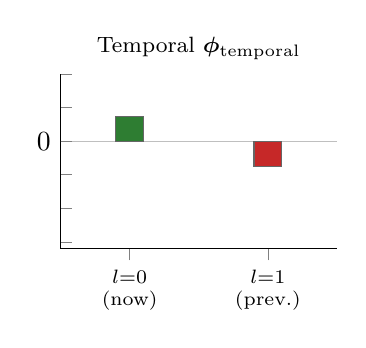
\begin{tikzpicture}
\begin{axis}[
  width=0.42\columnwidth, height=38mm,
  ybar, bar width=10pt, bar shift=0pt,
  symbolic x coords={l0,l1},
  xticklabels={$l{=}0$\\(now),$l{=}1$\\(prev.)},
  xticklabel style={font=\scriptsize, align=center},
  xtick={l0,l1},
  ymin=-0.32, ymax=0.20, ytick={-0.3,-0.2,-0.1,0,0.1,0.2},
  yticklabels={},
  title={\footnotesize Temporal $\boldsymbol\phi_{\mathrm{temporal}}$}, title style={yshift=-1.5mm},
  axis lines*=left, extra y ticks={0}, extra y tick style={grid=major},
  enlarge x limits=0.5]
\addplot[fill=posgreen, draw=black!60] coordinates {(l0,0.0741)};
\addplot[fill=negred, draw=black!60] coordinates {(l1,-0.0750)};
\end{axis}
\end{tikzpicture}
\caption{Explanation of the top-scored true anomaly on UCI-Message
($s^*=0.9965$). Green raises the anomaly score, red lowers it. Spatial values
sum each role over both lookback steps; $n_r$ is the neighbour of PageRank
rank $r$.}
\label{fig:example}
\end{figure}

An analyst reads it as follows. \emph{Spatially}, both endpoints push the score
up ($+0.161$, $+0.165$), while the top-ranked neighbour $n_1$ pulls it down
strongly ($-0.293$): this neighbour looks like normal context, so the alarm is
about the pair $(u,v)$ itself, not about a suspicious counterparty around it.
\emph{Temporally}, the current snapshot raises the score ($+0.074$) and the
previous one lowers it ($-0.075$): the interaction does not fit the pair's
recent history, so the anomaly appeared \emph{now}. A scalar score gives
neither answer. For the top alarms on the two Bitcoin datasets, the temporal
vector also favours the current snapshot ($+0.057$ vs.\ $+0.043$ on
Bitcoin-Alpha; $+0.018$ vs.\ $-0.012$ on Bitcoin-OTC).

\subsection{Computational Cost}
On a single CPU core (Google Colab), one explanation takes $0.18$\,s
($0.17$--$0.18$\,s across datasets), against $0.035$\,ms per edge for batched
TADDY inference. Gradient$\times$Input costs $0.004$\,s, and attention and
gradient norms are almost free. The cost of our method grows linearly with
$N_s$, since each coalition is one Transformer forward pass, and the $N_s$
passes can be batched on a GPU. This fits offline triage of the alarms an
analyst actually reviews, not scoring every edge in a stream.

% =============================================================================
\section{Discussion}
\label{sec:discussion}
% =============================================================================

\subsection{Why the Dual Decomposition Matters}
Any per-token score can be summed into spatial and temporal vectors. What our
framework adds is that the summed values are coalition-based marginal
contributions that satisfy the Shapley axioms (efficiency, symmetry, linearity,
null player) \cite{shapley1953value}, while gradients measure first-order
sensitivity and attention reflects internal focus rather than effect on the
output \cite{jain2019attention}. Table~\ref{tab:baselines} shows this
difference in practice: the tokens our method selects are the most necessary
ones (highest Comprehensiveness on every dataset).

\subsection{Why Post-Hoc?}
\label{subsec:posthoc}
We chose a post-hoc design on purpose. \textbf{Deployment:} practitioners often
have trained detectors they cannot retrain; intrinsic methods such as TGIB
\cite{seo2024tgib}, SIGNET \cite{liu2023signet} and DyExplainer
\cite{wang2023dyexplainer} change the training objective, which can change
detection. Our framework keeps $\Delta$AUC $=0$. \textbf{Separation of
concerns:} detection and explanation can be improved independently.
\textbf{Reuse:} the same procedure applies to any detector with a similar
token input.

\subsection{Applicability Beyond TADDY}
The framework needs only a token-based input and a forward pass from token
embeddings. It applies directly to other windowed Transformer detectors that
encode an edge as a token sequence, and the dual aggregation of
Eq.~\eqref{eq:decomp} only needs to know the role and time step of each player.
For models without explicit tokens, such as recurrent GNN detectors
\cite{zheng2019addgraph} or subgraph-based detectors \cite{cai2021strgnn}, the
players must be redefined (for example as nodes of the enclosing subgraph per
snapshot) and the neutral replacement must be chosen for that input space; this
is the main step needed to transfer the method. In social network operations,
the output answers the two questions moderators ask about an alert: \emph{who}
drove it, and \emph{when}.

\subsection{Borderline Detections and Negative Comprehensiveness}
\label{subsec:borderline}
For low-confidence true positives on Bitcoin-Alpha, Comprehensiveness is
negative ($-0.3995$): removing the top-$k$ tokens \emph{raises} the score. For
these borderline edges, the tokens with the largest $|\hat\beta|$ are those
that pull the score down, and the anomaly signal is spread across many tokens
rather than concentrated in a few. Such edges are better described by the whole
attribution vector than by a top-$k$ summary, and an analyst should read them
that way.

% =============================================================================
\section{Conclusion}
\label{sec:conclusion}
% =============================================================================
We introduced the first post-hoc explainability framework for TADDY-style
dynamic graph anomaly detectors. For each flagged edge it returns a spatial
vector (which roles drove the alarm) and a temporal vector (which snapshot),
with no change to detection. On the same trained models, it gives the most
necessary explanations of all baselines (highest Comprehensiveness on every
dataset, $p<10^{-10}$) and the best Fidelity where the metric is not saturated.
The ablation shows that its key ingredient is embedding-space masking, while the
sampler and kernel weights are replaceable. An evaluation over $2{,}621$ edges
and a worked example show how the two vectors support alarm triage, including
false alarms. The explainability gap is not unique to TADDY: it is the default
state of deep dynamic graph detectors, and the recipe used here (frozen model,
meaningful players, neutral replacement in the model's own input space)
offers a template for closing it.

% =============================================================================
\begin{thebibliography}{99}

\bibitem{akoglu2015graph}
L.~Akoglu, H.~Tong, and D.~Koutra, ``Graph based anomaly detection and
description: A survey,'' \emph{Data Mining and Knowledge Discovery}, vol.~29,
no.~3, pp.~626--688, 2015.

\bibitem{yu2018netwalk}
W.~Yu, W.~Cheng, C.~C. Aggarwal, K.~Zhang, H.~Chen, and W.~Wang, ``NetWalk: A
flexible deep embedding approach for anomaly detection in dynamic networks,'' in
\emph{Proc. ACM SIGKDD Int. Conf. Knowl. Discovery Data Mining}, 2018,
pp.~2672--2681.

\bibitem{zheng2019addgraph}
L.~Zheng, Z.~Li, J.~Li, Z.~Li, and J.~Gao, ``AddGraph: Anomaly detection in
dynamic graph using attention-based temporal GCN,'' in \emph{Proc. Int. Joint
Conf. Artif. Intell. (IJCAI)}, 2019, pp.~4419--4425.

\bibitem{cai2021strgnn}
L.~Cai, Z.~Chen, C.~Luo, J.~Gui, J.~Ni, D.~Li, and H.~Chen, ``Structural
temporal graph neural networks for anomaly detection in dynamic graphs,'' in
\emph{Proc. ACM Int. Conf. Inf. Knowl. Manage. (CIKM)}, 2021, pp.~3747--3756.

\bibitem{liu2021taddy}
Y.~Liu, S.~Pan, Y.~G. Wang, F.~Xiong, L.~Wang, Q.~Chen, and V.~C.~S. Lee,
``Anomaly detection in dynamic graphs via transformer,'' \emph{IEEE Trans.
Knowl. Data Eng.}, vol.~35, no.~12, pp.~12081--12094, 2023.

\bibitem{nekka2026survey}
I.~A. Nekka, H.~Seba, K.-W. Hidouci, and K.~Amrouche, ``Deep learning for
anomaly detection in dynamic graphs: A verified taxonomy, survey, and unified
benchmark,'' SSRN preprint 7339339, 2026. [Online]. Available:
\url{https://papers.ssrn.com/sol3/papers.cfm?abstract_id=7339339}

\bibitem{ranshous2016scalable}
S.~Ranshous, S.~Harenberg, K.~Sharma, and N.~F. Samatova, ``A scalable approach
for outlier detection in edge streams using sketch-based approximations,'' in
\emph{Proc. SIAM Int. Conf. Data Mining (SDM)}, 2016, pp.~189--197.

\bibitem{eswaran2018spotlight}
D.~Eswaran, C.~Faloutsos, S.~Guha, and N.~Mishra, ``SpotLight: Detecting
anomalies in streaming graphs,'' in \emph{Proc. ACM SIGKDD Int. Conf. Knowl.
Discovery Data Mining}, 2018, pp.~1378--1386.

\bibitem{yang2025generaldyg}
X.~Yang, X.~Zhao, and Z.~Shen, ``A generalizable anomaly detection method in
dynamic graphs,'' in \emph{Proc. AAAI Conf. Artif. Intell.}, 2025.

\bibitem{lou2023gady}
S.~Lou, Q.~Zhang, S.~Yang, Y.~Tian, Z.~Tan, and M.~Luo, ``GADY: Unsupervised
anomaly detection on dynamic graphs,'' \emph{arXiv preprint arXiv:2310.16376},
2023.

\bibitem{ying2019gnnexplainer}
Z.~Ying, D.~Bourgeois, J.~You, M.~Zitnik, and J.~Leskovec, ``GNNExplainer:
Generating explanations for graph neural networks,'' in \emph{Adv. Neural Inf.
Process. Syst. (NeurIPS)}, 2019.

\bibitem{luo2020pgexplainer}
D.~Luo, W.~Cheng, D.~Xu, W.~Yu, B.~Zong, H.~Chen, and X.~Zhang, ``Parameterized
explainer for graph neural network,'' in \emph{Adv. Neural Inf. Process. Syst.
(NeurIPS)}, 2020.

\bibitem{duval2021graphsvx}
A.~Duval and F.~D. Malliaros, ``GraphSVX: Shapley value explanations for graph
neural networks,'' in \emph{Proc. Eur. Conf. Mach. Learn. Knowl. Discovery
Databases (ECML-PKDD)}, 2021, pp.~302--318.

\bibitem{lundberg2017shap}
S.~M. Lundberg and S.-I. Lee, ``A unified approach to interpreting model
predictions,'' in \emph{Adv. Neural Inf. Process. Syst. (NeurIPS)}, 2017.

\bibitem{xia2023tgnnexplainer}
W.~Xia, M.~Lai, C.~Shan, Y.~Zhang, X.~Dai, X.~Li, and D.~Li, ``Explaining
temporal graph models through an explorer-navigator framework,'' in
\emph{Proc. Int. Conf. Learn. Represent. (ICLR)}, 2023.

\bibitem{chen2023tempme}
J.~Chen and R.~Ying, ``TempME: Towards the explainability of temporal graph
neural networks via motif discovery,'' in \emph{Adv. Neural Inf. Process. Syst.
(NeurIPS)}, 2023.

\bibitem{wang2023dyexplainer}
T.~Wang, D.~Luo, W.~Cheng, H.~Chen, and X.~Zhang, ``DyExplainer: Explainable
dynamic graph neural networks,'' \emph{arXiv preprint arXiv:2310.16375}, 2023.

\bibitem{seo2024tgib}
S.~Seo, S.~Kim, J.~Jung, Y.~Lee, and C.~Park, ``Self-explainable temporal graph
networks based on graph information bottleneck,'' in \emph{Proc. ACM SIGKDD
Conf. Knowl. Discovery Data Mining (KDD)}, 2024.

\bibitem{han2026explainable}
X.~Han, X.~Hu, C.~Ma, and X.~Shang, ``Explainable anomaly detection in dynamic
heterogeneous graphs via relation evolution,'' \emph{IEEE Trans. Knowl. Data
Eng.}, vol.~38, no.~5, pp.~2793--2806, 2026.

\bibitem{shapley1953value}
L.~S. Shapley, ``A value for $n$-person games,'' in \emph{Contributions to the
Theory of Games II}. Princeton, NJ, USA: Princeton Univ. Press, 1953,
pp.~307--317.

\bibitem{deyoung2020eraser}
J.~DeYoung, S.~Jain, N.~F. Rajani, E.~Lehman, C.~Xiong, R.~Socher, and B.~C.
Wallace, ``ERASER: A benchmark to evaluate rationalized NLP models,'' in
\emph{Proc. Annu. Meeting Assoc. Comput. Linguistics (ACL)}, 2020,
pp.~4443--4458.

\bibitem{jain2019attention}
S.~Jain and B.~C. Wallace, ``Attention is not explanation,'' in \emph{Proc.
Conf. North Amer. Chapter Assoc. Comput. Linguistics (NAACL)}, 2019,
pp.~3543--3556.

\bibitem{simonyan2014saliency}
K.~Simonyan, A.~Vedaldi, and A.~Zisserman, ``Deep inside convolutional
networks: Visualising image classification models and saliency maps,'' in
\emph{Proc. Int. Conf. Learn. Represent. (ICLR) Workshop}, 2014.

\bibitem{shrikumar2017deeplift}
A.~Shrikumar, P.~Greenside, and A.~Kundaje, ``Learning important features
through propagating activation differences,'' in \emph{Proc. Int. Conf. Mach.
Learn. (ICML)}, 2017, pp.~3145--3153.

\bibitem{wilcoxon1945}
F.~Wilcoxon, ``Individual comparisons by ranking methods,'' \emph{Biometrics
Bulletin}, vol.~1, no.~6, pp.~80--83, 1945.

\bibitem{liu2023signet}
Y.~Liu, K.~Ding, Q.~Lu, F.~Li, L.~Y. Zhang, and S.~Pan, ``Towards
self-interpretable graph-level anomaly detection,'' in \emph{Adv. Neural Inf.
Process. Syst. (NeurIPS)}, 2023.

\end{thebibliography}

\end{document}
